% !TEX root = ../main.tex
\pagebreak[0]
\section{Generating and verifying the certificate}\label{sec:generating-and-verifying-the-certificate}

The components of the preceding sections are combined in a single search
over $B_0$. Its result is a certificate: one record for every eliminated
box. The certificate is checked separately from the search that produced
it, and this check, together with the mathematics of the preceding
sections, proves \cref{thm:main}.

\subsection{Complete coverage and the main theorem}\label{subsec:complete-coverage-and-the-main-theorem}

\paragraph{The collection.}
The final collection has four components: the Domain component of
\cref{subsec:domain-component-skipping-boxes-outside-the-reduced-domain},
the Global component of \cref{sec:global-component}, the Local component of
\cref{sec:local-component}, and the Exotic component with the eight
covers of \cref{sec:square-and-pentagon-configurations,sec:arc-configurations,sec:endpoint-and-crossing-configurations}.
\Cref{tab:covers} lists the 38 zoom covers. The Local and Exotic
components work in the same way, by inclusion in a checked cover; we keep
them apart because the Local covers form one uniform family, indexed by
viewing rectangles, while each Exotic cover belongs to a particular
configuration. The components are tried in the order Domain, Exotic,
Local, Global, since the first three tests are fast and the Global
component's test is the most expensive.

\begin{table}[htbp]
\centering\small
\begin{tabular}{llllrr}
  \toprule
  Cover & No-fit set & Zooms & Section & Zoom cells & Records\\
  \midrule
  Local $0,\dots,29$ & aligned & tube (face zooms) & \ref{subsec:face-zooms-and-the-local-component} & 833 & 21{,}792\\
  square & aligned & point & \ref{subsec:eliminating-the-square-configuration} & 877 & 56\\
  pentagon & aligned & point & \ref{subsec:eliminating-the-pentagon-configuration} & 6{,}173 & 315\\
  arc$\pm$ & $\Pi_{\pm1}$ & tube & \ref{subsec:eliminating-arc-configurations} & 343, 288 & 135, 68\\
  endpoint$\pm$ & $\Pi_{\pm1}$ & point & \ref{subsec:eliminating-the-endpoint-configuration} & 305, 246 & 55, 23\\
  crossing$\pm$ & $\Pi_{\pm1}$ & point, hand-over & \ref{subsec:eliminating-the-crossing-configuration} & 1{,}431, 687 & 86, 58\\
  \bottomrule
\end{tabular}
\caption{The zoom covers of the Local component (first row) and of the
Exotic component, with the number of their terminal cells that carry
witnesses and the number of certificate records naming them. The pairs are
for $\sigma=1$ and $\sigma=-1$. The parameters of every cover are listed in
\cref{app:zoom-covers}.}
\label{tab:covers}
\end{table}

\paragraph{Records.}
A search box is named by its \emph{path}: the sequence of choices, $0$ for the
lower half and $1$ for the upper half, that leads to it from $B_0$ under the
cyclic bisection of \cref{subsec:boxes-subdivision-and-elimination}. A
certificate record consists of the path, the component that eliminated the
box, and the data its test needs: the violated inequality of $D$ for the
Domain component, the hole edge and plug vertex for the Global component,
and the zoom cover containing the box for the Local and Exotic
components. For example, the record with path \texttt{11} names the
viewing-triangle inequality: the box
$[1/3,2/3]\times[1/5,2/5]\times{[-2/5,2/5]}^3$ lies beyond the boundary
$\varphi s+\varphi^2t=1$.

\paragraph{Checking a certificate.}
A certificate is accepted when two checks succeed.
\begin{enumerate}
  \item \emph{Coverage.} The paths must be the leaves of a finite binary
    tree rooted at $B_0$: no path is a prefix of another, and every
    sequence of choices meets one of them after finitely many steps. The
    checker verifies this by reading the paths in order of increasing depth
    and, within a depth, in lexicographic order, while maintaining the list
    of boxes not yet accounted for; the list must be empty at the end.
  \item \emph{Records.} Each record's test is repeated exactly on its box:
    the Bernstein sign test of the named inequality, the Bernstein sign
    tests of the sixty gap polynomials, or the exact inclusion in the named
    cover's covered set. The covers themselves are rebuilt and all their
    cells checked, as described in \cref{app:zoom-covers}, before any
    record is read.
\end{enumerate}

\begin{proposition}[Complete coverage]\label{prop:complete-coverage}
  If both checks succeed, the boxes of the records cover $B_0$, and every
  box satisfies \cref{eq:box-elimination}.
\end{proposition}
\begin{proof}
  The children of a box cover it, so by induction on the tree, its leaves
  cover the root $B_0$. Each record passed its component's test, and the
  components are sound: the Domain component by
  \cref{subsec:domain-component-skipping-boxes-outside-the-reduced-domain},
  the Global component by \cref{prop:soundness-of-the-global-component},
  the Local component by \cref{prop:soundness-of-the-local-component}, and
  the Exotic component by
  \cref{prop:square-neighbourhood,prop:pentagon-neighbourhood,prop:arc-neighbourhoods,prop:endpoint-neighbourhoods,prop:crossing-neighbourhoods}.
\end{proof}

\begin{proof}[Proof of \cref{thm:main}]
  The final certificate passes both checks. If the RID were Rupert, a fit
  would exist and, by \cref{prop:representative-coverage}, a fit would lie
  in $D\subseteq B_0$. By \cref{prop:complete-coverage}, it would lie in an
  eliminated box, contradicting \cref{eq:box-elimination}.
\end{proof}

\paragraph{What the proof rests on.}
Unwinding the propositions cited above, the proof uses:
\begin{itemize}
  \item the reduction to the domain $D$: \cref{sec:geometric-formulation}
    and \cref{prop:representative-coverage}, with the symmetry data of
    \cref{app:symmetry-data-and-checks};
  \item the Bernstein sign test (\cref{lem:bernstein-sign-test}) and the
    exact arithmetic of \cref{sec:reduction-to-exact-arithmetic};
  \item the Domain and Global tests
    (\cref{subsec:domain-component-skipping-boxes-outside-the-reduced-domain,prop:soundness-of-the-global-component});
  \item the zoom lemma (\cref{lem:zoom-lemma}) with its two kinds of
    witnesses, gap polynomials and domain polynomials;
  \item the two no-fit sets: the aligned configurations
    (\cref{subsec:the-zoom-lemma}) and the arc planes
    (\cref{lem:arc-planes-contain-no-fit});
  \item the coverage lemmas for tube zooms, point zooms and the hand-over
    (\cref{lem:tube-coverage,lem:point-coverage,lem:hand-over}), which give
    the neighbourhood propositions of
    \cref{sec:local-component,sec:square-and-pentagon-configurations,sec:arc-configurations,sec:endpoint-and-crossing-configurations};
  \item a correct implementation of the two checks above, for which the
    independent checker described below provides a second implementation,
    and of the cover checks of \cref{app:zoom-covers}, which that checker
    takes as given and which the program's tests re-verify with independent
    reimplementations.
\end{itemize}
The list of touch configurations, the analyses of why finitely many cells
suffice, the floating-point proposals and the program that found the cells
are not needed.

\subsection{Implementation, execution, and reproducibility}\label{subsec:implementation-execution-and-reproducibility}

The search and the checker form one program, written in Rust, which
combines the performance needed for a search over hundreds of thousands of
boxes with a type system that keeps exact numbers, polynomials, boxes and
records strictly apart. Arbitrarily large integers and rationals come from
the standard \texttt{num} libraries; numbers of $\mathbb Q(\sqrt5)$,
polynomials in five variables and their Bernstein coefficients are
implemented in the program itself, as described in
\cref{sec:reduction-to-exact-arithmetic}. Floating point is used only to
choose which witness to try; every acceptance is decided exactly. The
search processes boxes in a fixed order, so its certificate does not depend
on the number of threads, and it can be interrupted and resumed from the
certificate alone.

The final search, on 16 threads of a workstation, evaluated 385,391 boxes
and wrote 192,696 records in about a minute; checking them takes about half
a minute. Most records are Global records (157,458); the Local, Domain and
Exotic components account for 21,792, 12,650 and 796.
\cref{fig:aligned-slice} shows how the components share a slice of the
configurations.

\begin{figure}[htbp]
\centering
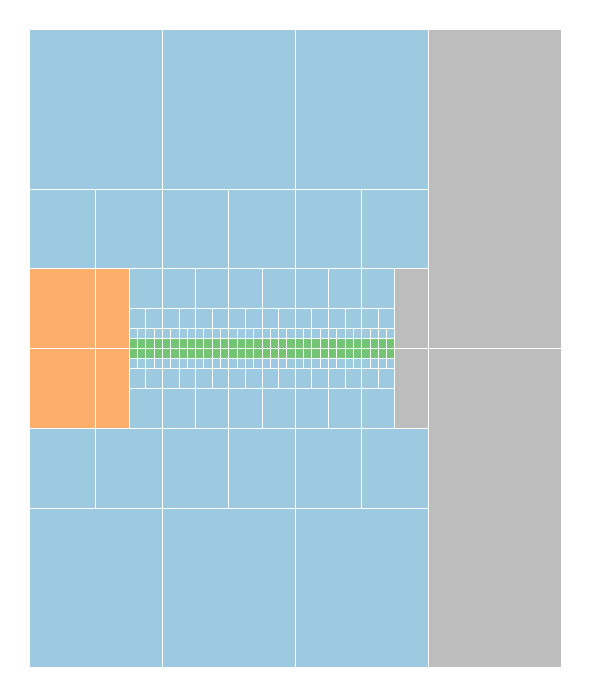
\includegraphics[width=0.5\linewidth]{figures/slice-aligned}
\caption{A slice of the final collection: $t=1/10$ and $r_1=r_2=0$, with $s\in[0,2/3]$ horizontally and $r_3\in[-2/5,2/5]$ vertically, halved alternately until one component eliminates each piece, and coloured by that component: \fc{Global}{light blue Global}, \fc{Local}{green Local}, \fc{Square}{light orange the square cover}, \fc{Domain}{grey Domain} (beyond the boundary of the viewing triangle). The Local component takes over in a thin band around $r_3=0$, where the configurations are nearly aligned. The search itself halves five-dimensional boxes.}
\label{fig:aligned-slice}
\end{figure}

\paragraph{Testing and validation.}
The program is tested extensively, with unit, integration and adversarial
tests of every part, including independent reimplementations of the exact
arithmetic, the zooms and the covers. Two experiments validate the
collection: every configuration of a list of 683 configurations chosen near
the touch configurations of the preceding sections has a neighbourhood
that the collection eliminates, and each component and cover is the only
one to eliminate the boxes around some configuration, so none of them is
redundant. Finally, an independent checker written in Python from the
definitions alone re-verified every record of the final certificate and its
coverage of $B_0$, taking the cells of the zoom covers as checked by the
program.

\paragraph{Reproducibility.}
The program, its zoom cover data, the final certificate and the
independent checker are available in the repository
\url{https://github.com/bence-hervay/nopert-rid}.
From its source directory, building the program
and running its check on the certificate repeats every test of
\cref{subsec:complete-coverage-and-the-main-theorem}; running the search
reproduces the certificate byte for byte. The SHA-256 hash of the final
certificate is
\texttt{df1f8dbab68b561f22fa9daeca48153d}\allowbreak\texttt{71bde7b6fba3345d9f6b7b8077df4b5f}.
